\chapter{Related work}

%TODO: longer

This chapter reviews approaches made towards handling Known-item Search (KIS) task and the recent approaches for user-friendly traverse through the immersive amount of the visual data.

In recent years, we witnessed a significant advancement in the solution for the KIS task. The scale of the solution's complexity for user interaction ranges from simple ones (e.g., sketching color blocks) with only a few descriptors to the ones which use recent advance in deep learning, as for concept labeling (i.e, naming objects).

Our goal is to perform known-item-search task on a set of videos. We perform a common simplification, replacing videos with the set of images. We do this, since we look for a particular scene, which can be also an image. This level of abstraction therefore corresponds to the searched query. Also, this allows us to use a potential of a common neural networks and other solutions presented for 2D data (images in our case). For this task we perform sampling over the videos. More information is available in section \ref{}\todo{fix}, where more details about the dataset are available.

\section*{Known-item-search Task}

Known-item-search task is present in many different situations. The tasks is to efficiently retrieve a known item in the dataset. For example, for a database of newspaper article we may use such retrieval tools to find a particular article we are interested in. Our thesis focuses on visual KIS task, specifically we retrieve images. For the setting we solve our task in exist even annual competitions to share the knowledge and the advancements. One of such is Video Browser Showdown \ref{}\todo{fix}, which is taking place since 2012. We review a few of the presented solutions to this task from the last VBS2019. We mainly follow the summarization in the \ref{}\todo{fix}

The most common approach at the VBS2019 were "Query by an Image" and "Concept Labeling". Query by an image, in this case, mostly refers to finding the most similar results from databse to given image. The downside of this approach is mainly the difficulty to obtain an image, which would be sufficiently similar to the searched one.

The second most used approach at VBS2019 was Concept Labelling. In this case, a user can describe the scene using the words. The database is pre-annotated with the vocabulary of present items. During the request, the algorithm checks the database for the presence of the searched concept. This approach has a limitation of the vocabulary size. Recent advancement in the textual annotation neural networks is nowadays able to describe thousands of different objects by words, but still, this may present on the limitation on rarely used objects or hard to describe objects.

One of the approaches presented and used is by creating a color sketch. The user colors the canvas with respect to the original searched scene. The database is then traversed on the correspondence of the colors to the particular part of the image. We see a significant advantage of this approach to distinguish between the key objects in the scene spatially.
 
Solving KIS task in VBS setting offers the option of using full video information and not only snapshots. This approach enhances the possibilities spectrum to Temporal Queries or Multimodal queries. Also, the solution included Optical Character Recognition (OCR) was presented. We present our solution as a possible enhancement of a complex system in order to create multiple search strategies based on user-preference. 

\section*{Traversion Approaches}

Since the KIS task is the task of two sides -- the algorithm and the user, it is essential to not forget about the easy to use interface. A good overview of the dataset may hide some deficiencies of the algorithm so that the user can still find the search scene. As the  (Evaluation of VBS ref)\todo{fix} shows, the most common approach is to show a 2D grid of images to the user. Several approaches also provide an easy way to play the original video as one of the most immersive ways we have encountered to traverse a grid of images is placing these images on the globe with the possibility of multiway traversing (TODO: ref). We aim to achieve a similar level of smooth traversing.

The traversing systems rely on effective visualization techniques on high-number feature spaces. These systems create mostly a 2D grid of the images based on the distance between the samples in high dimensionality space. Though, this high dimensionality space, often produced by neural networks, may not have feasible representation in 2D space based on the hidden features. This is often caused by a lack of understanding and representability of the deep features. We aim to test this feature reduction to the 2D test in our face experiment with the use of deep neural network features.

\section{Existing systems}

In the next section we shortly investigate on existing frameworks, which competed in the Video Browser Showdown.

\subsection{VIRET}

A framework named VIRET (\cite{lokovc2019framework, lokovc2019viret}) is successfully participating in the competitions for a several years now. The framework evolved in the years and now it offers a wide variety of the strategies for solving KIS task. VIRET also implements own strategy for a frame selection, which we also used for obtaining our images. As one of the biggest strategical advantages of the VIRET we consider a multi-modal queries with relevance scores and update of the queries based on the results. We take VIRET as our inspiration and we do not implement the same approaches as are already present in the VIRET. We focus on testing new alternatives.

\begin{figure}
    \centering
    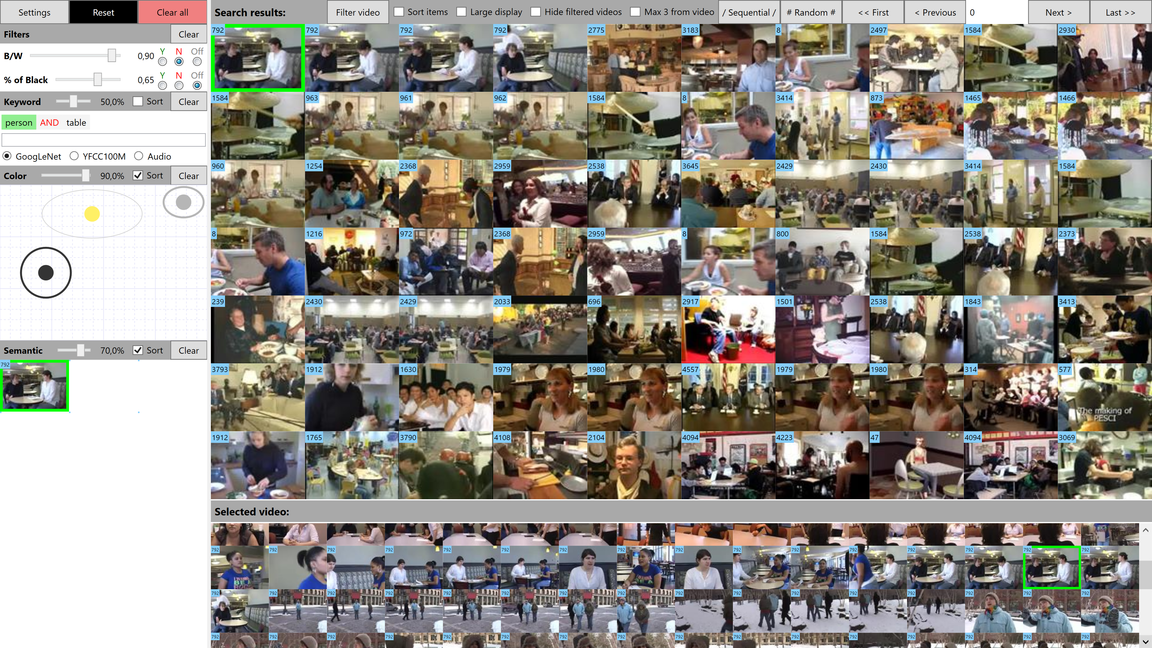
\includegraphics{img/viret_small.png}
    \caption{A sample search in VIRET framework. Source: https://videobrowsershowdown.org/hall-of-fame/}
    \label{fig:viret}
\end{figure}

\subsection{SOM Hunter}

A SOM Hunter (\cite{kratochvil2020som}) was for the first time introduced at the VBS2020. This tool is related to us, since it successfully proved using Self-organizing Maps for a use in a Known-item-search task. They train a small self-organizing map on the fly over only a sample of the dataset. This allows them to recreate the SOM based on the user interaction and train it on the fly. In our work we use the idea of training SOM, but compared to the SOM Hunter we will test creating a SOM only on the faces of the people.

\begin{figure}
    \centering
    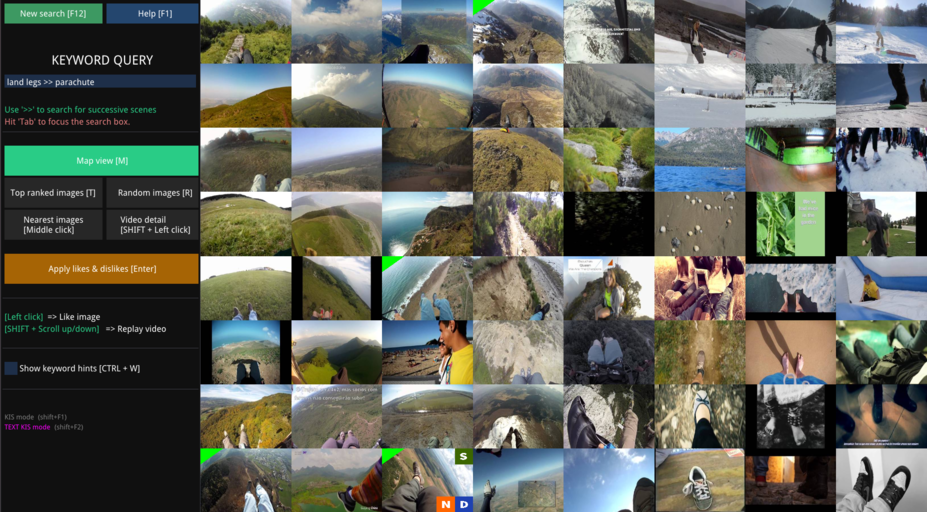
\includegraphics[width=0.99\linewidth]{img/som_hunter_small.png}
    \caption{A sample search in SOM Hunter. Source: https://videobrowsershowdown.org/hall-of-fame/}
    \label{fig:som_hunter}
\end{figure}

